\documentclass[draft, twoside=false]{scrbook}

% PACKAGES
\usepackage{typearea}
\usepackage{hyperref}
\usepackage[svgnames]{xcolor}
\usepackage{fontspec}
\usepackage{graphicx}
\usepackage{csquotes}
\usepackage[backend=biber, style=nature,maxcitenames=99]{biblatex}
\usepackage[acronyms, toc]{glossaries}
\usepackage{enumitem}
\usepackage{xparse}
\usepackage{cleveref}
\usepackage{siunitx}
\usepackage{microtype}
\usepackage{booktabs}

% CUSTOM COMMANDS
\DeclareDocumentCommand{\newdualentry}{ O{} O{} m m m m } {
  \newglossaryentry{gls-#3}{name={#5},text={#5\glsadd{#3}},
    description={#6},#1
  }
  \makeglossaries
  \newacronym[see={[Glossary:]{gls-#3}},#2]{#3}{#4}{#5\glsadd{gls-#3}}
}

% SETTINGS
\definecolor{UppsalaRed}{cmyk}{0,0.91,0.72,0.23}
\hypersetup{
    colorlinks=true,
    linkcolor=UppsalaRed,
    urlcolor=UppsalaRed,
    filecolor=UppsalaRed,
    citecolor=UppsalaRed
}
\defaultfontfeatures{Ligatures={Required, Common, TeX}}
\addbibresource{Half-Time Thesis.bib}
\DeclareBibliographyCategory{myworks}
\DeclareFieldFormat{labelnumber}{%
  \ifinteger{#1}
    {\number\numexpr#1-3\relax}
    {#1}}

\DeclareSIUnit{\litre}{\ell}
\DeclareSIUnit{\base}{bp}
\sisetup{
    per-mode = symbol
}

% METADATA
\title{Unraveling the Etiology of Complex Traits by Extending GWAS to Causal Inference and Copy Number Variation Analysis}
\author{Daniel Schmitz}
\date{2021-10-15}

% GLOSSARY
\makeglossaries
\newacronym{snp}{SNP}{single-nucleotide polymorphism}
\newacronym{cnv}{CNV}{copy-number variation}
\newacronym[
    plural=GWAS,
    firstplural=genome-wide association studies (GWAS)
    ]{gwas}{GWAS}{genome-wide association study}
\newacronym{ld}{LD}{linkage disequilibrium}
\newacronym[first=the Northern Swedish Population Health Study (NSPHS)]{nsphs}{NSPHS}{Northern Swedish Population Health Study}
\newacronym{pea}{PEA}{protein extension assay}
\newacronym{ukb}{UKB}{UK Biobank}
\newacronym{wgs}{WGS}{whole-genome sequencing}
\newacronym{smrt}{SMRT}{Single-Molecule Real-Time Sequencing}
\newacronym{t2d}{T2D}{type 2 diabetes}
\newacronym{bmd}{BMD}{bone mineral density}
\newacronym{iv}{IV}{instrumental variable}
\newacronym{maf}{MAF}{minor allele frequency}
\newacronym{qc}{QC}{quality control}
\newacronym{bmi}{BMI}{body-mass index}
\newacronym{hrt}{HRT}{hormone-replacement therapy}
\newacronym{oc}{OC}{oral contraceptive}
\newacronym{pc}{PC}{principal component}
\newacronym{shbg}{SHBG}{sex hormone-binding globulin}
\newacronym[
    plural = eQTL,
    firstplural = expression quantitative trait loci (eQTL)
    ]{eqtl}{eQTL}{expression quantitative trait locus}
\newacronym{gtex}{GTEx}{the Genotype-Tissue Expression project}
\newacronym{gsmr}{GSMR}{generalized summary-based Mendelian Randomization}
\newacronym{ivw}{IVW}{inverse-variance weighted}
\newacronym{gefos}{GEFOS}{the Genetic Factors for Osteoporosis Consortium}
\newacronym{or}{OR}{odds ratio}
\newacronym{dhea}{DHEA}{dehydroepiandrosterone}
\newacronym{cyp3a7}{CYP3A7}{cytochrome P450 3A7}
\newacronym[
    first=the International Classification of Diseases
    ]{icd}{ICD}{International Classification of Diseases}
\newacronym{icd9}{ICD-9}{\gls{icd}, revision 9}
\newacronym[first=revision 10 (ICD-10)]{icd10}{ICD-10}{\gls{icd}, revision 10}
\newacronym{bcac}{BCAC}{the Breast Cancer Association Consortium}
\newacronym{ecac}{ECAC}{the Endometrial Cancer Association Consortium}
\newacronym{ocac}{OCAC}{the Ovarian Cancer Association Consortium}
\newacronym{sv}{SV}{structural variation}
\newacronym{acgh}{aCGH}{array comparative genomic hybridization}
\newacronym{ngs}{NGS}{next-generation sequencing}
\newacronym{clr}{CLR}{continuous long read}
\newacronym[
    firstplural=small insertions and deletions (indels)
]{indel}{indel}{small insertion and deletion}
\newacronym{mr}{MR}{Mendelian Randomization}
\newacronym{wes}{WES}{whole-exome sequencing}
\newacronym{cn}{CN}{copy number}
\newacronym{sbs}{SBS}{sequencing by synthesis}
\newacronym{pcr}{PCR}{polymerase chain reaction}
\newacronym{pacbio}{PacBio}{Pacific Biosciences}

% START OF DOCUMENT
\begin{document}

\frontmatter
\newlength{\oldparindent}
\setlength{\oldparindent}{\parindent}

\parskip 6pt
\parindent 0pt

\begin{titlepage}
    \centering
    \makeatletter
    \LARGE \sffamily \@title

    \Large \rmfamily \@author

    \vspace*{\fill}
    
\includegraphics[width=.5\pagewidth]{img/UU_logo_4f_42.pdf}

    \vspace*{\fill}
    \normalsize
    \textbf{Half-Time Thesis} \\
    Department of Immunology, Genetics and Pathology,\\
    Science for Life Laboratory, Uppsala University

    \@date
    \makeatother
\end{titlepage}

{ % Nested in a group to reset typesetting
    \raggedright
    \textbf{Main Supervisor}\\
    Åsa Johansson, PhD\\
    Associate Professor \\
    Department of Immunology, Genetics and Pathology. Medical Genetics and Genomics, Science for Life Laboratory, Uppsala University, Sweden

    \textbf{Co-Supervisors}\\
    Torgny Karlsson, PhD\\
    Researcher \\
    Department of Immunology, Genetics and Pathology. Medical Genetics and Genomics, Science for Life Laboratory, Uppsala University, Sweden

    Adam Ameur, PhD \\
    Bioinformatician \\
    Department of Immunology, Genetics and Pathology, Uppsala Genome Center, Uppsala University, Sweden

    \textbf{Review Committee}\\
    Nils Landegren, PhD\\
    Associate senior lecturer/Assistant Professor\\
    Department of Medical Biochemistry and Microbiology, Comparative genetics and functional genomics, Uppsala University, Sweden.

    Tomas Bergström, PhD\\
    Researcher\\
    Department of Animal Breeding and Genetics; Molecular genetics, HgenLab, Sveriges Lantbruksuniversitet, Sweden

    Susanna Larsson, PhD\\
    Senior lecturer/Associate Professor\\
    Department of Surgical Sciences, Medical epidemiology, Uppsala University, Sweden

    % COPYRIGHT NOTICE
    \vfill
    \footnotesize
    © 2021 Daniel Schmitz

    This work is licensed under the Creative Commons Attribution 4.0 International License. To view a copy of this license, visit \url{http://creativecommons.org/licenses/by/4.0/}.
}

\chapter{Abstract}
    This is an abstract! And this is a \href{https://schmytzi.github.io/}{link}! There is also a \gls{mr} study.

\chapter{List of Publications}
This thesis is based on the following papers and projects, referred to in the text by their numbers.

\begin{enumerate}[label=\Roman*.]
    \item \fullcite{Schmitz2021} \addtocategory{myworks}{Schmitz2021}
    \item \fullcite{Johansson2021} \addtocategory{myworks}{Johansson2021}
    \item Characterizing Copy Number Variations using Next- and Third-Generation Sequencing and their Association with Plasma Biomarkers
    \item Unspecified
\end{enumerate}

\section*{Related Publications}
The following publications are not part of the main research project.
\begin{itemize}
    \item \fullcite{Kierczak2021} \addtocategory{myworks}{Kierczak2021}
\end{itemize}

\tableofcontents

\mainmatter
\glsresetall
\parskip 0pt
\parindent \oldparindent
\chapter{Introduction}
Since the first assembly of the human genome was published in 2001, numerous links between genetic variants and complex traits as well as diseases have been established \cite{Lander2001}.
Traditionally, \gls{snp} genotyping followed by \glspl{gwas} has been the way to go.
During recent years however, \gls{ngs} and even long-read sequencing have become increasingly mature and affordable.
This development allows not only for the genotyping of rare \glspl{snp}, but also the detection of large \glspl{sv}.
In addition to identifying genetic associations, post-\gls{gwas} analyses have been developed.
For instance, \gls{mr} studies allow researchers to establish relationships between traits or disease risk through the use of \gls{gwas} data.

\section{Genome-Wide Association Studies}
\Glspl{gwas} identify associations between genetic variants and phenotypes.
The majority of \glspl{gwas} investigate \glspl{snp} and \glspl{indel} for associations.
However, the method is not restricted to these kinds of variants.

To perform a \gls{gwas}, it is first necessary to genotype a large cohort of individuals.
Usually, this is done using \gls{snp} arrays, which only allow for the detection of previously identified variants but are generally cheap and reliable.
Other genotyping approaches which use \gls{ngs}, such as \gls{wgs} and \gls{wes}, have increased in popularity and have recently become feasible for large-scale studies.
After genotyping, \glspl{snp} that were not present on the genotyping array are often imputed from the ones that were present based on \gls{ld}.

Suitable phenotype for \gls{gwas} can be quantitative traits, e.g. height or levels of certain proteins in blood, or binary, e.g. the presence of a certain disease.
Data can be obtained in a variety of ways depending on the trait to be assessed.
The data can stem from measurements of blood samples, physical assessments, questionnaires or registries.
In addition to the specific phenotype the study is supposed to investigate, a number of other traits which might act as confounders are recorded.

After all data was collected, a \gls{gwas} identifies associations by applying a linear regression model for quantitative traits or a logistic model for binary traits.
This model uses the phenotype as response, each \gls{snp} as predictor and all phenotypes that might confound as covariates.
To control for multiple testing, an adjusted significance threshold of $p < 5 * 10^{-8}$ is commonly applied.
This is equivalent to adjusting for 1 million independent variants \cite{Belmont2005}.
Because of \gls{ld}, not all variants that pass genome-wide significance are reported.
Instead, variants that are close together, are clumped into one locus and only the variant with the strongest association, the \textit{lead \gls{snp}}, is reported.

Over the last two decades, \glspl{gwas} have enabled us to gain unprecedented insight into the genetic architecture of human diseases and complex traits.
Increasingly larger cohorts such as \gls{ukb} contributed to the continuously improving statistical power of \gls{gwas}, which accelerated this trend.
As of the time of writing, the GWAS Catalog---the largest database of \gls{gwas} results---contains 293,040 associations of \glspl{snp} and \glspl{indel} to phenotypes \cite{Buniello2019}.

\section{Mendelian Randomization}
In addition to elucidation the effect of \glspl{snp} on traits and disease risk, \gls{gwas} results can also be leveraged to infer associations between traits through an approach called \gls{mr} (\cref{fig:mr}).
\Gls{mr} studies apply a design based on randomized controlled trials to estimate the effect of an exposure $X$ on an outcome $Y$ using genetic variants as \glspl{iv}.
The underlying reasoning is that if there is a variant that affects the exposure, then it should indirectly and proportionally affect the outcome through the exposure.
In order for a variant to be a valid \gls{iv}, it must meet the following assumptions:
\begin{enumerate}[label=\bfseries IV\arabic*)]
    \item It is associated with the exposure.
    \item It is not associated with any confounders.
    \item It affects the outcome exclusively through the exposure.
\end{enumerate}
\Gls{mr} avoids problems of conventional observational studies such as reverse causation because its \glspl{iv} are assigned at conception.

\begin{figure}
    \centering
    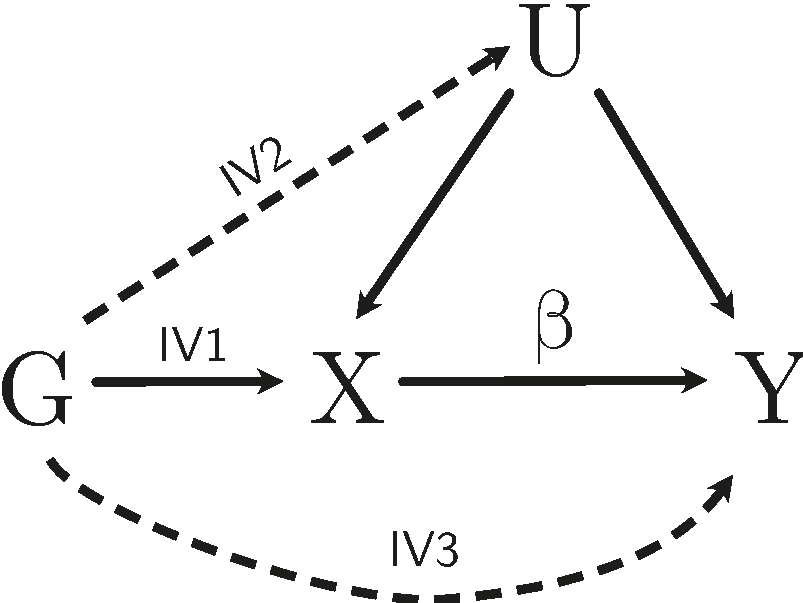
\includegraphics[width=.5\textwidth]{img/mr_graph.pdf}
    \caption{Graphical representation of the assumptions of \gls{mr}.
    The strength $\beta$ of the causal effect of $X$ on $Y$ is to be estimated.
    The genetic variants $G$ affect $X$ (IV1) but neither any confounders $U$ (IV2) nor $Y$ (IV3) directly.
    Original from \cite{J2015}.}
    \label{fig:mr}
\end{figure}

\begin{figure}
    \centering
    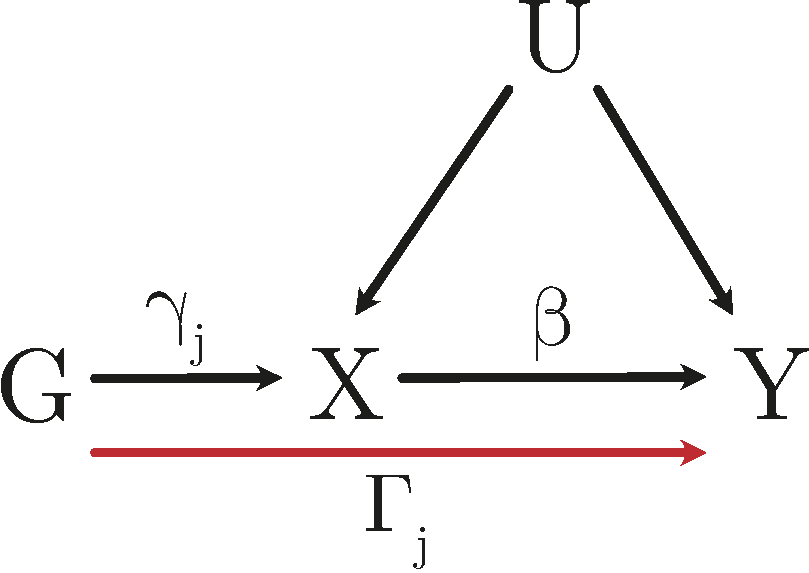
\includegraphics[width=.5\textwidth]{img/two_sample_mr.pdf}
    \caption{Graphical representation of the summary-based \gls{mr} approach.
        $\Gamma_j$ refers to the effect size estimated by a \gls{gwas}, which only assesses association, not causality, and not a pleiotropic effect of $G$ on $Y$.
        The effect $\beta$ can be calculated according to $\beta=\frac{\Gamma_j}{\gamma_j}$.
    }
    \label{fig:two-sample-mr}
\end{figure}

\begin{figure}
    \centering
    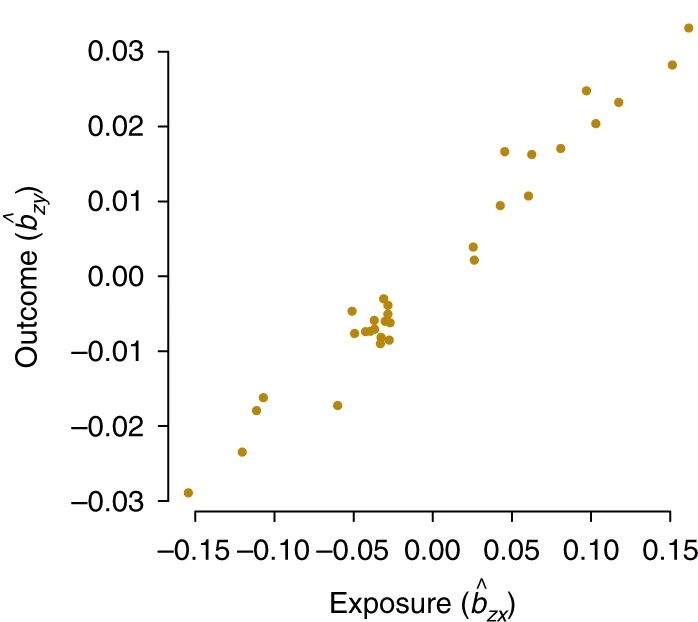
\includegraphics[width=.5\textwidth]{img/two_sample_mr_plot.png}
    \caption{Example of a two-sample \gls{mr} result.
    The x-axis shows the estimated effect of the \glspl{iv} on the exposure.
    The y-axis shows the effect on the outcome.
    The effect of the exposure on the outcome is equal to the slope of the linear regression.
    Adapted from \cite{Zhu2018}.}
    \label{fig:twosample-example}
\end{figure}

There are two major designs for \gls{mr} studies \cite{Burgess2019}.
One-sample \gls{mr} uses exposure and outcome data from the same cohort.
This allows for an easy study design, because you only need to measure an additional phenotype, but it might not always be possible to perform these measurements 

Two-sample \gls{mr} studies on the other hand use \gls{gwas} summary statistics from two different cohorts, one for the \gls{snp} effects on the exposure and one for the effects on the outcome, respectively.
Thanks to platforms like the GWAS Catalog and MR Base, summary statistics to use for two-sample \gls{mr} studies are easily available.
Often, genotyped or imputed \glspl{snp} are not the same between studies.
This makes it necessary to find proxy \glspl{snp} as replacement for lead \glspl{snp} that are not present in both studies' data.

\Gls{mr} studies can either be individual-based, which predict the exposure measurement for each individual based on their alleles and use this prediction as a predictor for the outcome, or summary-based, i.e. use effect estimates from previous \gls{gwas}.
The summary-based approach has become the more popular one, thanks to the wide availability of summary statistics online.
In short, this approach estim ates $\beta$ based on the observed effect $\gamma_j$ of the variant $G_j$ on $X$ and its effect $\Gamma_j$ on $Y$ (\cref{fig:two-sample-mr}).
If $X$ has a causal effect on $Y$, then the calculated $\beta$ should be constant for all $G_j$ (\cref{fig:twosample-example}).

There are multiple algorithms to estimate the causality between $X$ and $Y$ based on summary statistics.
They differ in weights they apply to \glspl{iv} and their ability to account for outliers or invalid instruments.
The most commonly used methods include \textit{weighted median} and \textit{\gls{ivw}}, which apply different weights to \glspl{iv} in the model and assume no directional pleiotropy, which occurs when the combined pleiotropic effects of the chosen \glspl{iv} do not add up to zero \cite{Burgess2013,Bowden2016}.
However, the MR-Egger method can take directional pleiotropy into account, but its use is discouraged in one-sample studies \cite{Bowden2015,Bowden2017}.
Finally, \gls{gsmr}, which allows for the detection and removal of pleiotropic \glspl{iv}, has become a popular method for \gls{mr} studies \cite{Zhu2018}.

\section{Copy Number Variations}
Despite the advances in the statistical power of \glspl{gwas}, only a fraction of observed heritability of many traits can be explained by \glspl{snp}.
The 1000 Genomes Project estimated in 2015 that 99.9\% of variants present in a typical human genome are \glspl{snp} and \glspl{indel} \cite{Auton2015a}.
However, they note that another kind of variation, \glspl{sv}, which are variants that affect more than \qty{50}{\base}, cover a larger fraction of the genome.
Another study from the same year found that \glspl{sv} account for approximately 13\% of genetic variation in humans \cite{Sudmant2015}.
Nonetheless, only few studies have investigated associations between \glspl{sv} and diseases or complex traits.

A big group of \glspl{sv} that has received more attention are \glspl{cnv}.
A \gls{cnv} is a variant that affects the number of copies, i.e. the \gls{cn}, of a genomic sequence (\cref*{fig:cnv}).
Short \glspl{cnv} have well established links to diseases such as Huntington's Disease and Fragile X Syndrome \cite{MacDonald1993,Verkerk1991}.
However, associations of longer \glspl{cnv} spanning multiple \si{\kilo\base} or even \si{\mega\base} are not well studied.

\begin{figure}
    \centering
    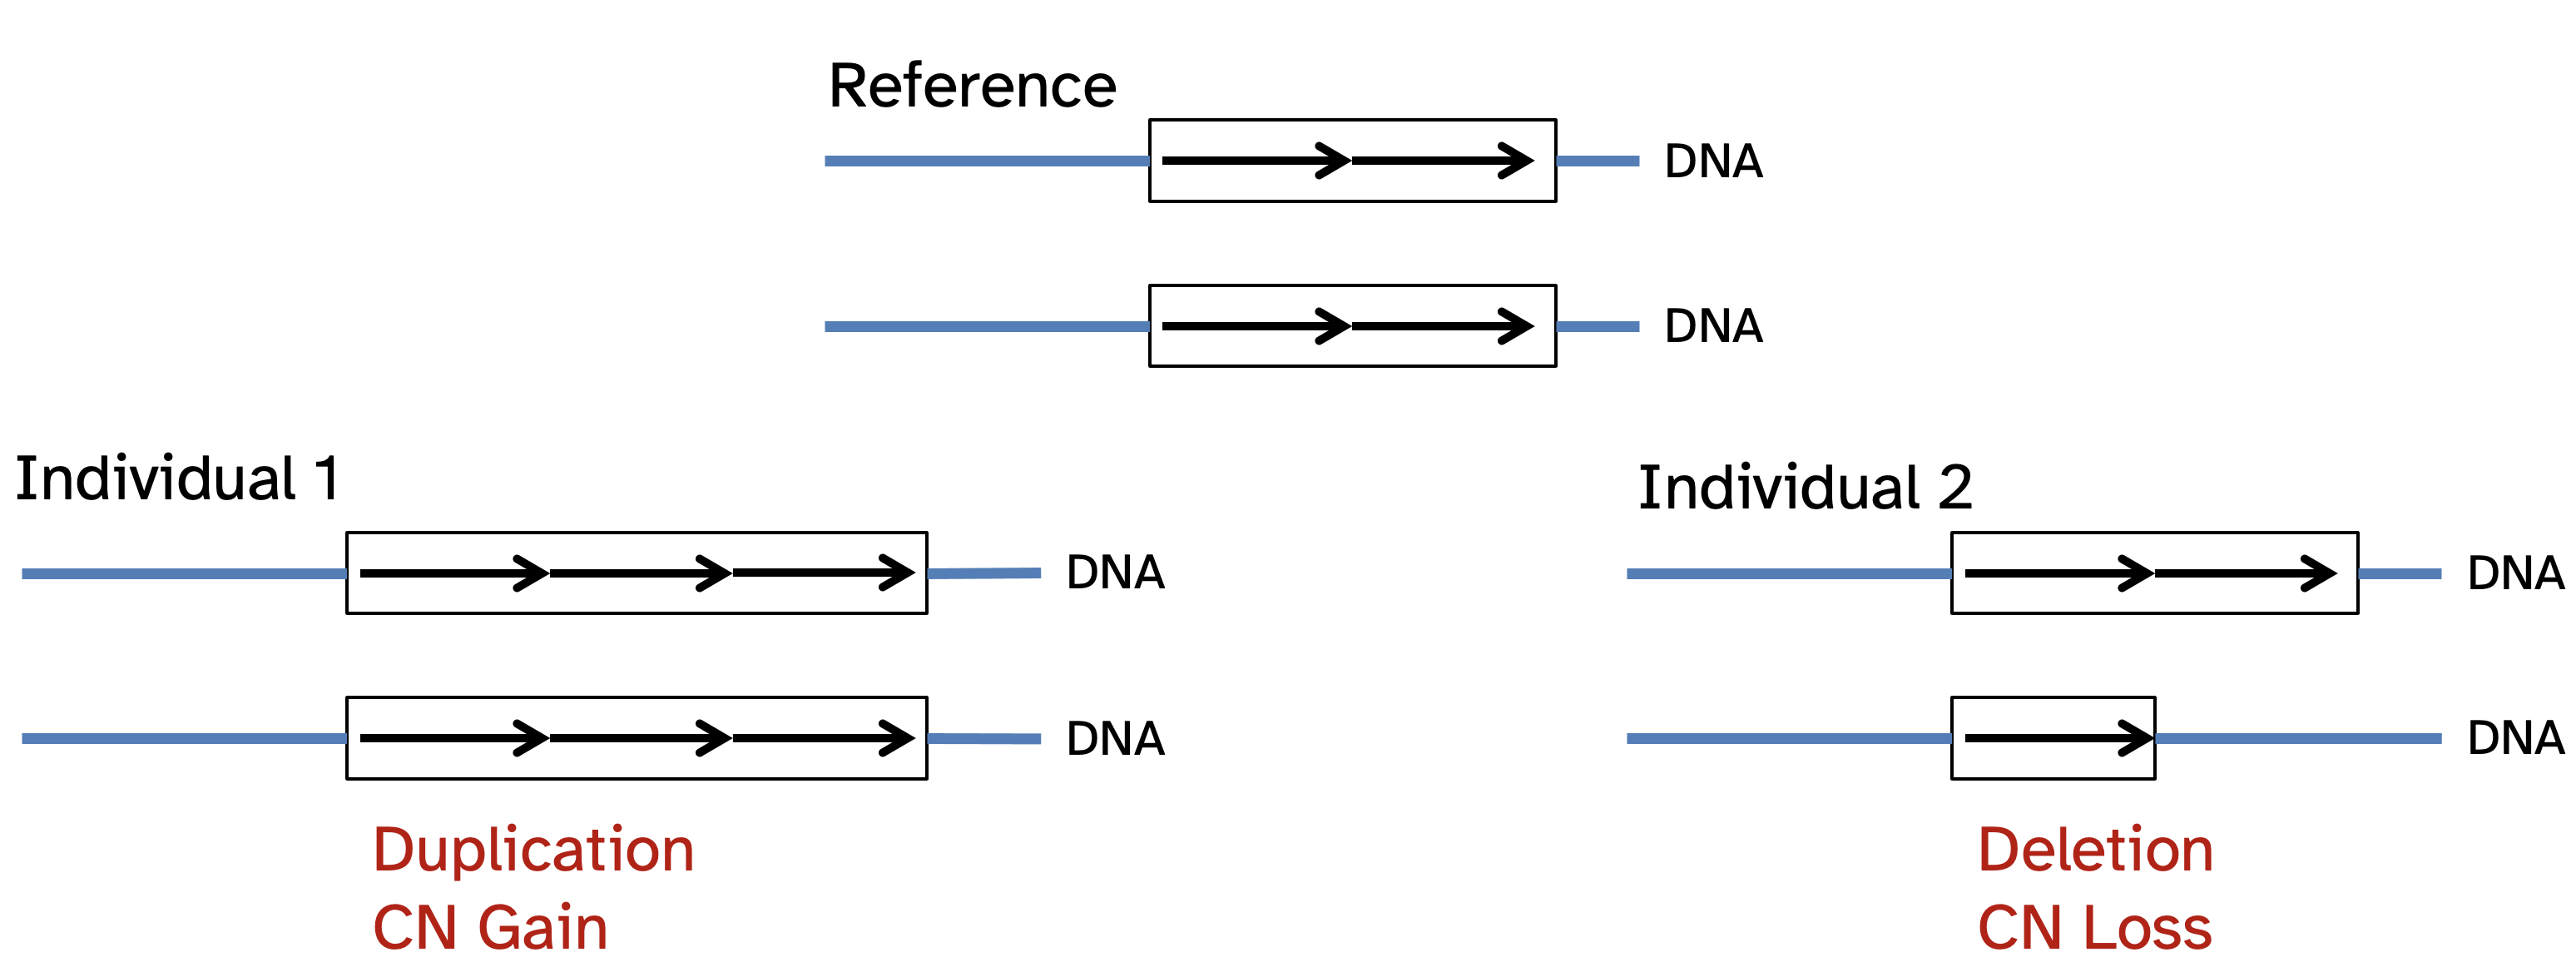
\includegraphics[width=\textwidth]{img/cnv_example.png}
    \caption{Example of a \gls{cnv}.
        Each arrow represents a copy of the sequence of interest.
        There is one copy in the (haploid) reference.
        In a diploid individual, this corresponds to \gls{cn} 2 (Individual 1).
        Individual 2 is homozygous for two copies of the sequence (\gls{cn} 4).
        An increase in the number of copies is called a \textit{duplication} or \textit{\gls{cn} gain}.
        Individual 3 has lost a copy of the sequence on one chromosome (\gls{cn} 1).
        This is called a \textit{deletion} or \textit{\gls{cn} loss}.}
        \label{fig:cnv}
\end{figure}

Despite their clinical significance, research into the effects of \glspl{cnv} on risk of disease and health-related traits is still lacking.
One important reason for the lack of research on the effects of \glspl{cnv} is the fact that they are hard to detect.
Most \gls{cnv} studies use microarray-based technologies such as \gls{acgh}.
However, these lack the ability to detect novel signals and have a limited resolution.
Common array-based workflows can only detect \glspl{cnv} with a size of at least \qty{8}{\kilo\base}, on average \cite{Quenez2020}.
Thanks to improving quality and cost of \gls{wgs}, the interest in \glspl{cnv} has increased dramatically, as this approach allows for the detection of \gls{cnv} loci not covered before.

\section{Sequencing Technology}
Sequencing technology has changed a lot over the last two decades.
While most of the Human Genome Project's first assembly was sequenced using Sanger sequencing, this technology proved to be too expensive and slow to allow for widespread use for human genomics \cite{Lander2001}.

Over the following years, technological advances enabled the emergence of a high-throughput sequencing, or \gls{ngs}.
These technologies allow to sequence billions of bases at a time while reducing cost.
Over the years, Illumina and their technology based on \gls{sbs} have become the market leader in this segment.
Their platform produces short paired-end reads with a usual length of around \qty{150}{\base} and leverages increasing computational power to align these short reads to the human genome.
While Illumina sequencing is highly accurate for the detection of \glspl{snp} and \glspl{indel}, they are too short to reliably represent large \glspl{sv}.
Moreover, the need for amplification via \gls{pcr} of the DNA to be sequenced makes Illumina sequencing vulnerable to \gls{pcr} amplification bias.
This leads to low coverage in regions with very high or low GC content \cite{Aird2011}.

Several approaches for \gls{cnv} detection have been developed for short-read alignments.
In general, these can be divided into two major groups: depth-based methods (e.g. \textsf{CNVnator} \cite{Abyzov2011b}), which identify \glspl{cnv} through regions of abnormally high or low coverage, and read-based methods (e.g. \textsf{Manta} \cite{Chen2016a}), which rely on anomalies in fragment size and read-pair orientation.

Recently, third-generation sequencing technologies, in particular \gls{pacbio} \gls{smrt} sequencing and Oxford Nanopore, have matured and become usable for larger research projects.
They are able to produce longer reads than previous technologies.
\Gls{smrt} reads usually range between \qtyrange{15}{20}{\kilo\base}, while Nanopore can produce reads of up to \qty{4}{\mega\base} \cite{Wenger2019,Payne2019}.
Furthermore, amplification-free protocols have been developed for long-read sequencing, which avoid the issues caused by \gls{pcr} amplification bias \cite{Hoijer2018}.
However, they suffer from low read accuracy, which makes them less suitable for \gls{snp} calling \cite{Rang2018}.

Several \gls{sv} callers exist for long-read alignments.
These include \textsf{Sniffles}, \textsf{SVIM} and \gls{pacbio}'s own \textsf{PBSV} \cite{Heller2019a,Sedlazeck2018a}.
They differ in how they incorporate \gls{sv} signatures from single reads and clusters of reads.
Furthermore, \textsf{PBSV} is the only caller to directly report \glspl{cnv} and \glspl{cn}.

\section{Study Cohorts}
\subsection{UK Biobank}
\Gls{ukb} is a long-time cohort study comprising about 500,000 participants born between 1939 and 1970 that were recruited from 2006 to 2010.
Extensive information on lifestyle and anthropometric traits was collected.
Participants left blood samples that were used for diverse measurements, including hormone levels, as well as genotyping of approximately 800,000 \glspl{snp}.

\subsection{Northern Swedish Population Health Study}
e employed \gls{nsphs}, a cohort study consisting of approx. 1000 individuals from two municipalities in northern Sweden, as the base cohort of our study.
Blood samples were collected on site and immediately frozen at \qty{-70}{\celsius}.
\Gls{wgs} was performed on an Illumina HiSeq X platform according to manufacturer specification with a target coverage of 30$\times$ \cite{Ameur2017}.
After \gls{qc} and mapping to reference genome GRCh37, 1021 individuals remained.

We measured 438 plasma biomarkers measured using Olink \gls{pea} in 903 individuals.
Of these, 982 individuals passed \gls{qc} for all protein measurements.
Overall, there were 872 individuals passing both genotype and protein \gls{qc}.



\chapter{Project I}
{
    \parindent 0pt \color{gray}
    Contributions: performed data analysis and interpretation, generated figures, wrote the manuscript
}

\section{Background}
Estrogen, which is generally known as the primary female sex hormone, is responsible for the female reproductive system's development.
Furthermore, it regulates the menstrual cycle and plays a critical role in male sexual function \cite{Bates2013b,Hess1997b}. 
Among the three major forms of estrogen: estrone, estradiol and estriol, estradiol is the most potent and abundant \cite{Thomas2013c}.

Estradiol levels have been associated with several conditions, incl. deep vein thrombosis, cancers and \gls{t2d} \cite{Cauley1999a, Rosendaal2003b,Vikan2010}.
In particular, declining estradiol levels after menopause have been linked to reduced \gls{bmd} and, in turn, higher risk of osteoporosis \cite{Riggs1998a,Longo2012a}.

Previous \glspl{gwas} for estradiol levels have been performed in sex-stratified populations comprising up to 11,000 people, most often of European descent \cite{Pott2019e,Chen2013d,Liu2013b,Prescott2012f,Eriksson2018b}.
Additionally, a recent study in \gls{ukb} identified strong sex-specific genetic effects on testosterone but excluded associations with estradiol measurements because of their strong link to age at menopause \cite{Ruth2020d}.

Apart from \glspl{gwas}, the causal effect of hormones on diseases and disease risk has been assessed using \gls{mr} \cite{Eriksson2018b,Ruth2020d, Nethander2018a}.
While previous \gls{mr} studies identified a beneficial effect of estradiol on \gls{bmd} in males, there have been no such studies in females due to failure to identify valid instruments for \gls{mr} analyses \cite{Eriksson2018b, Nethander2018a}.

In this project, we aimed to identify variants affecting estradiol.
Additionally, we aimed to estimate the causal effect of estrogen on \gls{bmd}.

\section{Methods} \label{sec:p1methods}
We used data from \gls{ukb} to perform this study.
We used \gls{snp} data imputed using UK10K and 1000 genomes phase 3 reference panels, containing 93,093,070 \glspl{snp} overall.
After \gls{qc}, 361,975 individuals remained, of which 167,168 were male and 194,807 were female.

Only measurements that were taken from blood samples given at the first visit at the assessment center were included in the analysis.
Estradiol was measured by two-step competitive analysis using a Beckman Coulter Unicel Dxl 800.
The assay had a lower detection limit of \qty{175}{\pmol\per\litre}, which is above the normal range for serum estradiol concentrations in postmenopausal females (0 -- \qty{73.4}{\pmol\per\litre}) \cite{Nakamoto2010a}.
Because of the resulting large fraction of measurements below detection limit, estradiol levels were analyzed as a binary phenotype (above/below detection limit).

We performed two sex-stratified \glspl{gwas} using logistic regression with additive genetic modeling in \textsf{PLINK~2}.
We included age, \gls{bmi}, the first ten genetic \glspl{pc} and the used genotyping array as covariates, as well as a binary indicator for the used genotyping array to control for batch effects.
For females, we included \gls{hrt}, \gls{oc} use (never/ever/current), number of live births, menopausal status and whether they had had a hysterectomy, too.
We identified lead \glspl{snp} by applying conditional analyses until no significant hits remained.
We tested all lead \glspl{snp} for sex-specific effects by including an interaction term in the logistic model.
We performed four sensitivity analyses.
We stratified females into pre- and postmenopausal, excluded all patients with cancer diagnoses and included testosterone and \gls{shbg} levels as covariates.
Lastly, we applied a Tobit-I model, which allowed us to incorporate quantitative estradiol measurements where available.

We annotated our lead \glspl{snp} to their closest genes and identified possible functional effects using \textsf{HaploReg} version 4.1 \cite{Ward2012}.
We used data from \gls{gtex} to check for overlap with known \glspl{eqtl} \cite{Carithers2015}.
Lastly, data from the GWAS Catalog was used to search for prior functional annotation of our lead \glspl{snp}.

To estimate the effect of estradiol on \gls{bmd}, we performed a one-sample \gls{mr} analysis in males and females separately using our \gls{gwas} lead \glspl{snp} as \glspl{iv}.
Due to the low number of significant associations in the female cohort, we applied a relaxed significance threshold ($p < 10^{-7}$) tp increase the number of available \glspl{iv}.
\Gls{bmd} had been recorded using an ultrasound measurement and converted to T-Scores, i.e. the number of standard deviations the measurement differed from the patient's sex's mean. 

The main \gls{mr} analysis was performed using the \textsf{gsmr} package, version 1.0.8 \cite{Zhu2018}, which implements the \gls{gsmr} method.
We performed sensitivity analyses using the \gls{ivw}, weighted median and MR-Egger methods implemented in the \textsf{TwoSampleMR} package in \texttt{R} \cite{Hemani2018}.
Additionally, we performed a two-sample \gls{mr} test using the aforementioned methods with summary statistics for lumbar-spine \gls{bmd} from \gls{gefos} \cite{Estrada2012}.
Because \gls{gefos} had used a different imputation panel than \gls{ukb}, we revised the set of \glspl{iv}.
For each locus, we selected the most significant common \gls{snp} in \gls{ld} with our lead \gls{snp}.

\section{Results and Discussion}
\label{sec:p1discussion}
\subsection{Genotyping and Estradiol Measurements}
After genotype and estradiol \gls{qc}, 147,690 males remained, of whom 134,323 had estradiol below and 13,367 above detection limit (\qty{175}{\pmol\per\l}).
Slightly more females (163,985) remained, with 126,524 individuals having estradiol levels below detection limit and 37,461 above.
Only 9.1\% of males and 7.9\% of postmenopausal females had detectable estradiol levels, while 71.9\% of premenopausal females had measurements.

The low number of individuals with available measurements was due to the estradiol assay having a low sensitivity.
A more sensitive method would have been preferable.
For future studies aiming to elucidate the genetic factors behind estradiol levels, we would recommend the usage of an assay that can detect lower concentrations of estradiol.
In fact, estradiol assays with a detection limit as low as \qty{2}{\pg\per\ml} ($\approx$ \qty{7.34}{\pmol\per\l}) are available to researchers \cite{Travison2014}.

\subsection{GWAS Results}
We found 15 loci on 14 chromosomes to be significantly associated ($p < 5*10^{-8}$) with estradiol levels, of which 13 were specific to males, one (\textit{MCM8}) specific to females and one (\textit{CYP3A7}) shared between both sexes.
We identified one conditional hit each on chromosomes 2 and 15.
12 of our \gls{gwas} hits had already established links to estradiol or steroid-hormone metabolism.
An additional analysis using a sex-genotype interaction term revealed strong sex-specific effects.
Most of the loci we identified have previously established links to steroid-hormone metabolism, including synthesis, conversion, transport and elimination of steroid hormones.

After stratification of the female cohort into pre- and postmenopausal, we identified one locus (\textit{CYP3A7}) with significantly different effects between the two strata.
Removal of all participants with previous cancer diagnoses did not lead to a change in our primary \gls{gwas} results.
Lastly, adjusting our model for testosterone and \gls{shbg} levels caused the loci \textit{SHBG} and \textit{FKBP4} to lose genome-wide significance with lower effect estimates.
The loci \textit{AR} and \textit{UGT3A1} lost significance, too, but the estimated \glspl{or} did not differ significantly.

Thanks to our secondary analysis using Tobit-I-modeling, we could somewhat ameliorate the problem of missing estradiol measurements.
This statistical approach allowed us to make use of estradiol measurements where available while still retaining information about which missing values were below detection limit.
This analysis mostly agreed with our primary results.
Among males, 11 \glspl{snp} and all \glspl{snp} that were significant for females replicated.
The effect estimates we obtained from our Tobit model were comparable to previous \glspl{gwas} of estradiol measurements \cite{Prescott2012f, Eriksson2018b,Pott2019e}.
We argue therefore that Tobit modeling provides a viable approach for \glspl{gwas} of phenotypes for which high-sensitivity assays might not be available.

\textit{CYP3A7} was significant in both males and females, indicating an important role in estrogen metabolism in both sexes.
Interestingly, it was also the only gene to have significantly different effects in pre- and postmenopausal females.
\textit{CYP3A7} encodes \gls{cyp3a7}, which metabolizes a precursor of both androgens and estrogens: \gls{dhea} \cite{Ohmori1998}.
Up to 75\% of estrogens in premenopausal women are derived from \gls{dhea} and after menopause, it is the main precursor of androgens and estrogens \cite{Simpson2001}.
When adjusting for \gls{shbg} and testosterone, \textit{CYP3A7}'s effect disappeared in females.
These findings point to \gls{cyp3a7} fulfilling different functions for steroid-hormone metabolism in males and females.

Interestingly, \textit{ABO}, the gene responsible for the ABO blood groups, was associated with estradiol levels in males \cite{Ogasawara1996}.
Our effect allele (rs657152-A) is in \gls{ld} with rs8176719-G, which is present in individuals that do not have blood type O.
This indicates that people with blood type O have higher estradiol levels.

\subsection{MR Results}
We estimated the causal effect of estradiol on \gls{bmd} using \gls{mr} in males and for the first time in females.
We included up to 16 \glspl{snp} in our \gls{mr} analyses, a large increase from five \glspl{iv} from previous studies \cite{Nethander2018a}.
Our effect estimates were higher in females than in males, indicating that bone metabolism depends more on estradiol in females.
This agrees with the rapid decline of \gls{bmd} after menopause and subsequently the prevalence of osteoporosis in postmenopausal women.

We identified few significant loci in females, which led to only four \glspl{iv} being included in the \gls{mr}.
Estradiol levels in women vary wildly during the menstrual cycle, making the genetic effect hard to estimate.
Furthermore, estrogen levels drop after menopause and are mostly determined by the time that has passed since the last menstruation \cite{Richardson2020}.
Both of these aspects probably limited the power of our \gls{gwas}.
Moreover, the low number of \glspl{iv} in our \gls{mr} analyses could have made the results unstable and increased the risk of them being affected by pleiotropy.

In summary, we identified genetic loci that affect estradiol levels with strong sex-dependent effects.
We showed the causal effect of estradiol on \gls{bmd}, supporting \gls{hrt} as a preventative treatment of osteoporosis.
Our findings confirm established medical research as well as provide insight into the metabolism and function of estrogens.

\chapter{Project II}
{
    \parindent 0pt \color{gray}
    Contributions: generated figures, performed estradiol \gls{gwas}, contributed to and reviewed the manuscript, interpreted data
}

\section{Background}
Despite its important functions for development and health, estrogen has been associated with a number of diseases.
Higher estradiol levels have been associated with an increased risk of breast cancer in pre- as well as postmenopausal women \cite{Key2013,Kaaks2005,Zhang2013,Kaaks2005a}.
However, a definite causal relationship, i.e. whether high estradiol levels increase the risk of breast cancer or cancer progression causes estradiol levels to rise, has not been established.

Two other major forms of cancer---endometrial and ovarian cancer---have clearly established links to estradiol levels \cite{Brinton2014,Mungenast2014}.
Progesterone has been shown to have a protective effect against these kinds of cancer, which is why menopausal \gls{hrt} is often combined with progesterone.
The same effect can be observed for \glspl{oc} because they contain a synthetic form of progesterone---progestin \cite{Karlsson2021,Iversen2017}.

Despite the clearly established association between the aforementioned cancers and estrogen, it remains unclear whether the body's own production of estrogen has an effect on cancer risk.
\gls{mr} is a commonly used approach to establish such a causal link.
In fact, there has been one study that used one \gls{snp} as \gls{iv} to estimate the effect of endogenous estradiol on endometrial cancer \cite{Thompson2016}.
No previous \gls{mr} studies concerning the effect of estradiol on breast or ovarian cancer have been published.

In this project we aimed to estimate the causal effect of estrogen on women's risk of breast, endometrial and ovarian cancer using the genetic instruments we identified in project I.

\section{Methods}
We used female participants from \gls{ukb} as the base cohort for this study.
Genotype and sample \gls{qc} were discussed in \hyperref[sec:p1methods]{Project~I}, as we used the effect estimates for estradiol from that study.

We assessed cancer incidence using diagnoses from hospital stays, death and cancer registries as well as answers from verbal interviews and touchscreen questionnaires.
Diagnoses were encoded as codes from \gls{icd9} and \gls{icd10}.
Breast cancer was represented by codes 174 (\gls{icd9}) and C50 (\gls{icd10}), ovarian cancer by codes 183 (\gls{icd9}) and C56 (\gls{icd10}) and endometrial cancer by \gls{icd10} code C541.
Most cases were recorded in the cancer register.
However, data from before 1995 was lacking.
Therefore, we had to rely on self-reported data for these cases.

We estimated the effects of our estradiol \glspl{iv} on risk for all three cancers using \textsf{PLINK 2}.
We applied a logistic model with additive effects with the following covariates: age, \gls{bmi}, genetic \glspl{pc} 1--10, \gls{hrt} use (never/ever/current), \gls{oc} use (never/ever/current), number of live births, menopausal status, whether the participant had undergone a hysterectomy and a binary indicator for the used genotyping array.

To infer the effect of endogenous estradiol on cancer risk, we performed a one-sample \gls{mr} analysis using our computed effect estimates and a two-sample \gls{mr} analysis, where we used publicly available \gls{gwas} data for \gls{snp} effects on cancer risk.
The main analyses were performed using the \texttt{R} package \textsf{gsmr} version 1.0.8 \cite{Zhu2018}.
We used the \texttt{R} package \textsf{MendelianRandomization} for sensitivity analyses, using the included methods: robust \gls{ivw}, weighted median and MR-Egger \cite{Olena2017}.
Effect estimates for breast cancer were taken from summary statistics published by \gls{bcac}, whose study included 122,977 breast-cancer cases and 105,974 healthy individuals of European origin \cite{Michailidou2017}.
Endometrial-cancer estimates were taken from a \gls{gwas} published by \gls{ecac} \cite{OMara2018}.
After removing individuals from \gls{ukb}, 12,720 cases and 46,126 controls of European ancestry remained.
Summary statistics for ovarian-cancer risk were taken from a study by \gls{ocac} including 25,509 cases of epithelial ovarian cancer and 40,491 controls \cite{Phelan2017}.

\section{Results and Discussion}
After \gls{qc}, 209,877 female \gls{ukb} participants remained, of which 13,179 had previously received a diagnosis of breast cancer, 1,981 of endometrial cancer and 1,477 of ovarian cancer.
Among the four chosen \glspl{iv}, two were nominally associated ($p_{adj} < 0.05$) with breast cancer and one \gls{iv} was associated with endometrial cancer.
In the summary statistics used for the two-sample \gls{mr}, one \gls{iv} was associated with ovarian cancer and one with endometrial cancer.
The \gls{snp} rs10638101 was missing in \gls{bcac}'s summary statistics and had therefore be substituted by the proxy rs897797, which was in perfect \gls{ld} ($R^2 = 1$).

\begin{table}[]
    \centering
    \begin{tabular}{@{}lllll@{}}
        \toprule
                                    & \multicolumn{2}{c}{\textbf{One-Sample}}                                              & \multicolumn{2}{c}{\textbf{Two-Sample}}                                             \\ 
                                    & \textbf{\begin{tabular}[c]{@{}l@{}}OR \\ (95\% CI)\end{tabular}}  & \textbf{P-value} & \textbf{\begin{tabular}[c]{@{}l@{}}OR \\ (95\% CI)\end{tabular}} & \textbf{P-value} \\
                                    \midrule
        \textbf{Breast Cancer}      & \begin{tabular}[c]{@{}l@{}}1.30       \\ (1.07 -- 1.57)\end{tabular} & 0.0074           & \begin{tabular}[c]{@{}l@{}}1.55\\ (0.91 -- 2.65)\end{tabular}       & 0.11             \\
        \textbf{Ovarian Cancer}     & \begin{tabular}[c]{@{}l@{}}1.19\\ (1.03 -- 1.38)\end{tabular}        & 0.018            & \begin{tabular}[c]{@{}l@{}}1.20\\ (0.99 -- 1.46)\end{tabular}       & 0.066            \\
        \textbf{Endometrial Cancer} & \begin{tabular}[c]{@{}l@{}}2.01\\ (1.21 -- 3.31)\end{tabular}        & 0.0065           & \begin{tabular}[c]{@{}l@{}}1.45\\ (1.14 -- 1.83)\end{tabular}       & 0.0022\\
        \bottomrule
        \end{tabular}
    \caption{\Gls{mr} results from our main analysis with \gls{gsmr}.}
    \label{tab:cancer_mr}
\end{table}

In our primary analysis using \textsf{gsmr}, we identified a causal effect of estradiol on breast-cancer and endometrial-cancer risk, both in the one-sample and the two-sample analyses (\cref{tab:cancer_mr}).
We did not detect a causal relationship for ovarian cancer.
In the sensitivity analysis, the MR-Egger method reported a significant intercept for the two-sample \gls{mr} of endometrial cancer, which is an indication of directional pleiotropy.
However, MR-Egger controls for this kind of pleiotropy.
Given that the effect estimate was significant, and its direction was consistent with all over approaches, we did not see evidence of strong pleiotropy.

\subsection{Cancer-Specific Results}
Our first \gls{iv} was annotated to \textit{CYP3A7}, which was discussed in \cref{sec:p1discussion}.
It had a nominally significant association to breast and endometrial cancer in \gls{ukb}, \gls{bcac} and \gls{ecac}.
\Gls{iv} number 2 was \textit{MCM8}, which has a strong association to age at menopause \cite{Chen2014}.
\textit{MCM8} was nominally associated with breast cancer in \gls{ukb} and \gls{bcac} and with endometrial cancer in \gls{ecac}.
Although we had not adjusted the estradiol \gls{gwas} for age at menopause, an analysis including only postmenopausal women and with age at menopause as covariate did not result in a significantly different effect estimate.
This suggests that the effect is not confounded by age at menopause.
Our third \gls{iv}, \textit{ASCL1}, has a previously established association to tumor progression in lung adenocarcinoma  and survival in patients with ovarian cancer \cite{Miyashita2020,Moore2017}.
It was nominally associated with risk for ovarian cancer in \gls{ocac}.
Our last \gls{iv}, \textit{TMEM1150B}, has an established association with age at menopause and menarche \cite{Stolk2012,Pickrell2016}.
It was significantly associated with breast cancer in \gls{ukb} and \gls{bcac}.

Our analyses showed no significant causal effect on estradiol on ovarian cancer.
However, the effect estimates from both the one- and two-sample tests showed a consistent effect direction and the result from the two-sample \gls{mr} would have passed a one-sided test (\cref{tab:cancer_mr}).
Therefore, we cannot conclude that there is no causal effect of estradiol on ovarian cancer.
However, we can safely say that the observed effect is weaker than the effects on breast and endometrial cancer \cite{Trabert2016,Key2011,Rodriguez2019}.

\subsection{Limitations}
Our \gls{mr} study was still limited by the overall small set of four \glspl{iv}.
This made our study vulnerable to directional pleiotropy.
In particular, the MR-Egger intercept of our two-sample analysis for endometrial cancer showed indications of pleiotropy.
Once larger cohorts or more quantitative estradiol measurements are available, it should be possible to identify more \glspl{iv} and alleviate this problem.
Furthermore, estradiol levels fluctuate wildly in women over the course of the menstrual cycle.
This and the strong correlation between estradiol levels in postmenopausal women and time since menopause make the detection of genetic \glspl{iv} complicated.

In summary, we identified a causal effect of estradiol on the risk of breast and endometrial cancer using a \gls{mr} approach in \gls{ukb}, \gls{bcac} and \gls{ecac} cohorts.
Our findings support prior research regarding the carcinogenic effects of estrogen.
Further research on the mechanism by which estrogens influence cancer development is needed, however.

\chapter{Project III}
{
    \parindent 0pt \color{gray}
    Contributions: analysed the long-read data, generated figures, wrote the manuscript
}

\section{Background}
Despite the success of \gls{ngs}, it is difficult to accurately detect \glspl{cnv} using this approach because the reads generated by \gls{ngs} are shorter than most \glspl{cnv}.
However, the advent of third-generation sequencing technologies such as \gls{pacbio} \gls{smrt} enables the generation of reads long enough to directly sequence long \glspl{sv} and improve mapping accuracy.

In this project, the aim was to identify \glspl{cnv} using \gls{wgs} and investigate if \gls{cnv} polymorphisms are associated with levels of plasma protein levels.
Moreover, we aimed to explore the application of long-read sequencing for the characterization of \glspl{cnv}.

\section{Methods}
We called \glspl{cnv} using \textsf{CNVnator}, a read-depth based method for \gls{cnv} detection \cite{Abyzov2011b}.
This tool calls \glspl{cnv} by dividing the genome into non-overlapping bins and identifying those bins that received abnormally high or low coverage.
The bin sizes were determined for each individual separately.
To facilitate association testing, we aligned the detected \glspl{cnv} to non-overlapping genomic windows of \qty{200}{\base}.
If a sample had a \gls{cnv} overlapping with a given window, we set that window's copy number appropriately.
Lastly, adjacent windows that had consistent copy numbers across individuals were merged to make up the final \glspl{cnv}.

We identified copy number-biomarker associations using a linear regression model (\texttt{glm} function in \texttt{R} version 4.3.4).
We included sex and age as covariates and applied an adjusted significance threshold of \(p < 4.79*10^{-9}\), which corresponds to the general significance threshold of $p < 0.05$ adjusted for 10,438,413 tests (438 proteins $\times$ 23,831 \glspl{cnv}).

We selected 15 individuals to be resequenced using \gls{pacbio} \gls{smrt} sequencing based on five \gls{cnv} that showed strong associations, were highly polymorphic and included both deletions and duplications (\cref{tab:cngwas}).
The individuals were chosen to capture as many \glspl{cn} as possible.
Long-read sequencing was performed on a \gls{pacbio} SEQUEL II system in \gls{clr} mode according to manufacturer specification.
\gls{pacbio}'s tool chain automatically mapped all reads to GRCh38.
Therefore, we had to extract the reads and remap them to GRCh37 using \textsf{pbmm2} version 1.4.0 to enable comparison between long-read and short-read data.
We called \glspl{sv} using three different tools: \textsf{SVIM} v1.4.2, \textsf{Sniffles} v1.0.12 and \textsf{PBSV} v2.4.0.

\section{Results and Discussion}
\begin{table}[]
    \begin{tabular}{@{}lrrrrrr@{}}
        \toprule
        \textbf{Biomarker} & \textbf{Chr} & \textbf{Start} & \textbf{End} & \textbf{Beta} & \textbf{SE} & \textbf{P Value} \\
        \midrule
        GPNMB    & 2  & 89,613,000  & 89,613,200  & -9.91E-01 & 1.56E-01 & 3.33E-10 \\
        PD-L2    & 3  & 98,411,600  & 98,411,800  & 4.09E-01  & 4.47E-02 & 3.92E-19 \\
        IL-18    & 5  & 70,393,100  & 70,393,300  & 4.18E-01  & 5.61E-02 & 2.38E-13 \\
        ST1A1    & 16 & 28,613,645  & 28,613,845  & 7.86E-01  & 6.93E-02 & 1.61E-27 \\
        hOSCAR   & 19 & 54,558,900  & 54,559,100  & -7.21E-01 & 6.27E-02 & 1.61E-28 \\
        \midrule
        CD48     & 1  & 158,867,600 & 158,867,800 & -2.82E-01 & 4.71E-02 & 3.15E-09 \\
        FCRLB    & 1  & 161,640,580 & 161,640,780 & 6.17E-01  & 9.11E-02 & 2.42E-11 \\
        LY9      & 1  & 179,455,600 & 179,455,800 & 5.36E-01  & 8.86E-02 & 2.17E-09 \\
        ICAM-2   & 3  & 98,410,600  & 98,410,800  & 6.48E-01  & 3.95E-02 & 5.67E-53 \\
        Siglec-9 & 3  & 98,411,800  & 98,413,400  & 6.82E-01  & 4.17E-02 & 3.48E-52 \\
        CD200R1  & 3  & 98,411,800  & 98,413,400  & 5.08E-01  & 4.45E-02 & 3.71E-28 \\
        VEGFR-3  & 3  & 98,414,600  & 98,414,800  & 5.96E-01  & 4.17E-02 & 1.10E-41 \\
        ICAM-3   & 3  & 98,899,900  & 98,900,100  & 3.96E-01  & 5.52E-02 & 1.45E-12 \\
        AMBP     & 5  & 745,070     & 745,270     & -2.84E-01 & 4.51E-02 & 5.05E-10 \\
        MIC-AB   & 6  & 32,496,600  & 32,496,800  & 6.19E-01  & 6.69E-02 & 3.35E-19 \\
        CCL19    & 6  & 32,522,200  & 32,522,400  & -4.67E-01 & 5.37E-02 & 1.93E-17 \\
        FR-gamma & 11 & 63,443,100  & 63,445,300  & -1.03E+00 & 9.83E-02 & 5.17E-24 \\
        FR-gamma & 11 & 67,331,355  & 67,331,955  & -1.23E+00 & 1.03E-01 & 1.64E-30 \\
        CNTN1    & 12 & 45,909,600  & 45,909,800  & -2.85E-01 & 4.69E-02 & 1.73E-09 \\
        CCL4     & 17 & 36,392,670  & 36,394,670  & 1.45E-01  & 2.29E-02 & 4.65E-10 \\
        CCL15    & 17 & 39,210,800  & 39,211,000  & -9.21E-01 & 1.23E-01 & 1.45E-13 \\
        SMPD1    & 19 & 35,863,600  & 35,863,800  & 3.69E-01  & 6.08E-02 & 1.97E-09 \\
        MIA      & 19 & 41,381,925  & 41,385,125  & -1.23E+00 & 1.69E-01 & 8.58E-13 \\
        hK11     & 19 & 51,508,940  & 51,510,740  & 1.41E+00  & 2.22E-01 & 3.84E-10 \\
        WFDC2    & 20 & 44,204,435  & 44,205,035  & 4.17E-01  & 6.81E-02 & 1.37E-09 \\
        \bottomrule
    \end{tabular}
    \caption{\Gls{cn}-\gls{gwas} results.
        The \glspl{cnv} in the top section were used to select the 15 individuals for resequencing.}
    \label{tab:cngwas}
\end{table}

Overall, 872 individuals had both genotyping and protein data which passed \gls{qc}.
\textsf{CNVnator} reported 243,987 \glspl{cnv}, which after post-processing resulted in 23,831 variants to be included in our analysis.
We found 30 \glspl{cnv} to be associated with 17 biomarkers (\cref{tab:cngwas}).

The quality of our long-read sequencing results was mixed.
While most samples received high coverage, in three cases less than half of all ZMWs produced high-quality reads.
The \gls{cnv} on chromosome 2 was not called by any of our long-read callers.
The \gls{cnv} on chromosome 3 was only detected by \textsf{SVIM}, which also called all copy numbers in accordance with \textsf{CNVnator}.
The \gls{cnv} on chromosome 5 was not detected in the long-read data.
The coverage in this region was spotty at best, in both Illumina and \gls{smrt} sequencing data.
This might be caused by the large number of repetitive elements and consequently low mappability in this region.
The \gls{cnv} on chromosome 16, which was exclusively called as a duplication by \textsf{CNVnator}, was not detected by any long-read caller.
However, \textsf{SVIM} called many smaller insertions in this region, which mapped well to repetitive elements.
This suggests that \textsf{CNVnator} might indeed have picked up on these repetitive elements and merged them into one big \gls{cnv} down the line.
The \gls{cnv} on chromosome 19 was consistently detected by all callers.

In general, deletions seem easier to detect and verify than duplications.

\section{Future Work}
This project has not concluded fully.
To make use of the results we have got so far, it would be interesting to investigate the detected \glspl{cnv} for effects of known functional elements in the genome.
This would help elucidate the pathways through which they affect their associated proteins.

Moreover, the data we alreay have might allow us to identify \glspl{snp} that tag or are in \gls{ld} with \glspl{cnv} of interest.
This might enable the creation of a larger imputation framework for \glspl{cnv} by use of \gls{ngs}-derived \gls{snp} data.

\chapter{Project IV}
\section{Future Work}
The research question that will be investigated in project IV has not been set, yet.
There are a few different projects that might be viable.
In general, further research into \glspl{cnv} and/or long-read sequencing, possibly as an extension of project III, sound interesting.

It might be worthwhile to develop a method that allows for easier \gls{cnv} validation.
So far, this is a manual process, which is very time-consuming.
Devising such a method would also benefit future research in this field.
However, it is difficult to exactly formalize when a \gls{cnv} can be considered validated.
For instance, the \glspl{cnv} that were called in short-read data but presented as groups of short duplications in long-read data are problematic cases.
While the \glspl{cnv} that were originally called did not validate \textit{per se}, there were in fact smaller variants that just happened to present as one large \gls{cnv}.
One could argue that this can still be considered a positive result that would not be trivial to detect.

We might be able to further elucidate the nature of the detected \glspl{cnv} by assembling the genomes of the individuals we sequenced using \gls{smrt} technology or a combination of both sequencing techniques.
No long-read \gls{sv} caller, except for \textsf{PBSV}, actually reports \glspl{cnv} as such and consequently, \glspl{cnv} and \glspl{cn} have to be inferred from the variants they do report, such as duplications, insertions and breakends.
An assembly might allow us to characterize the copy numbers and break points better.


\chapter{Concluding Remarks}
We investigated the role of genetic variants in human diseases through methods that supplement, complement and extend conventional \glspl{gwas}.
We identified the effect of genetic variants on estradiol levels and demonstrated the causal effect of estrogen on \gls{bmd} and certain cancers.
Furthermore, we identified \glspl{cnv}, which are not covered by common \glspl{gwas}, and characterized their association with plasma protein biomarkers.

While \glspl{gwas} have enabled groundbreaking research in the field of genetic epidemiology, it is becoming more apparent that there is a large part of heritability of certain traits and disease risk that they cannot explain.
To increase their statistical power, increasingly larger cohorts are needed.

Variants such as \glspl{cnv} are generally hard to detect and quantify.
Short-read sequencing, which has driven down cost and allowed for the detection of rare \glspl{snp} not covered by \gls{snp} arrays, has issues correctly capturing large \glspl{sv}.
This is in part due to their size but also due to many \glspl{sv} being hard to map because they lie in regions with many repeats or low complexity.

Long-read sequencing promises to ameliorate many problems of short reads but is still too expensive to be used in the same extent.
While these sequencing technologies have made considerable advances over the last few years, there are no universally accepted standards like for short-read sequencing and \gls{gwas} \cite{DeCoster2021}.

The improving accuracy and cost of \gls{wgs}, along with novel approaches such as haplotype-resolved and telomere-to-telomere assemblies, will make it possible to gain even deeper insights into the genetic architecture of human health \cite{Logsdon2021,Porubsky2021}.

\backmatter

\chapter{Acknowledgements}

\printglossary[type=\acronymtype]

\printglossary

\printbibliography[notcategory=myworks]
\end{document}